\stopallthesefloats
\subsection{On-Demand Cache Coherence}
\begin{figure}
\begin{center}
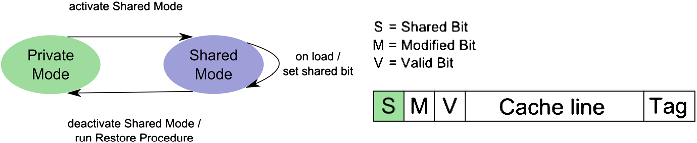
\includegraphics[width=\textwidth]{\chapterdirectory/figure/handling_it/odc2.pdf}
\end{center}
\caption{Overview of ODC\textsuperscript{2}, as seen in \cite{doi:10.1002/cpe.3172}.}%
\label{fig:handling_it:odc2}
\end{figure}

\cite{doi:10.1002/cpe.3172} presents ODC\textsuperscript{2} (On-Demand Coherent
Cache), a strategy to limit the interference of cache coherence on the
execution of real-time software (see Figure~\ref{fig:handling_it:odc2}). The
general idea is to have software delimit sections during which they access
shared data (\textit{Shared Mode}), and to have that shared data be evicted
from the cache as soon as the software leaves the section (\textit{Restore
Procedure}). Any new data loaded during Shared Mode is marked as being
\textit{shared} in the cache line, making their Shared data cannot be accessed
outside of these sections, which makes the code outside these coherence enabled
sections (called \textit{Private Mode}), much simpler to analyze.

A follow-up paper, \cite{Py2015.1}, performs the WCET analysis of some well
established algorithms (Dijkstra algorithm, Fast Fourier Transform, Matrix
Multiplication) by modifying an existing WCET computation framework (OTAWA) to
add support to ODC\textsuperscript{2}. The resulting WCET is compared with the
ones obtained when using no caches, when using \textit{Magic} (cache coherence
without any cost, which represents the best theoretical performance), and an
approach that simply invalidates the full cache upon entering any
synchronization point. The results show, somewhat unsurprisingly,
ODC\textsuperscript{2} obtains a lower computed WCET than the other approaches,
\textit{Magic} excepted.
